\section{Architecture and \\Problem Formalization}
In this section, we formalize the technical challenges addressed in this work.

\subsection{Problem 1. Cleanable Private Views}
The first problem that we address is to develop a $\epsilon$-local differentially private mechanism that allows for local cleaning.
Given a dirty relation $R$, the set of numerical attributes $A$, discrete attributes $D$, and a partition set of the discrete attributes $G$, \textbf{find a $\epsilon$-local differentially private transformation $T(\cdot)$ such that errors can be detected in $V=T(R)$ with an probability of $1-\alpha$ for any $\alpha \in (0,1)$.}

In our motivation, we alluded that the solution to this problem is a multi-column generalization of Warner's randomized response model.
However, there are few new issues, practical and theoretical, that we will subsequently address.
First, what is the dependence on the dataset size, and how many records are needed before the mechanism provides meaningful results.
Next, how do we ensure that randomization preserves enough structure such that the cleaners can still be used, i.e., preserve the domain of $g_i$.
Finally, how should we handle the numerical attributes.

\subsection{Problem 2. Cleaning and Aggregates}
The next problem that we explore is data cleaning and aggregate query result estimation on cleaned private views of data.
Let $V$ be a private relation and let $V_{clean}$ be a cleaned private relation after applying local cleaners.
For a \sumfunc, \countfunc, \avgfunc aggregate query $f$ with predicates, \textbf{estimate the result of the aggregate query $f$ with confidence intervals.}

The PrivateClean problem describes query processing on cleaned private relations. 
It turns out that the data cleaning operations change the statistical properties of the
randomization and these will have to be incorporated into the estimates.
Furthermore, we analyze two theoretical problem settings the asymptotic case and the finite sample case.

\subsection{Architecture}
Figure \ref{architecture} describes the architecture of \sys.
The system is initialized with a view of a database $R$, and \sys applies a randomized transformation and releases the private view.
\sys provides an API that allows for users to estimate aggregate query results using the private data after a restricted number of data cleaning operations.
The estimator manages the provenance of rows in the cleaned private view to correspond them with rows prior to cleaning.

\begin{figure}[t]
\centering
 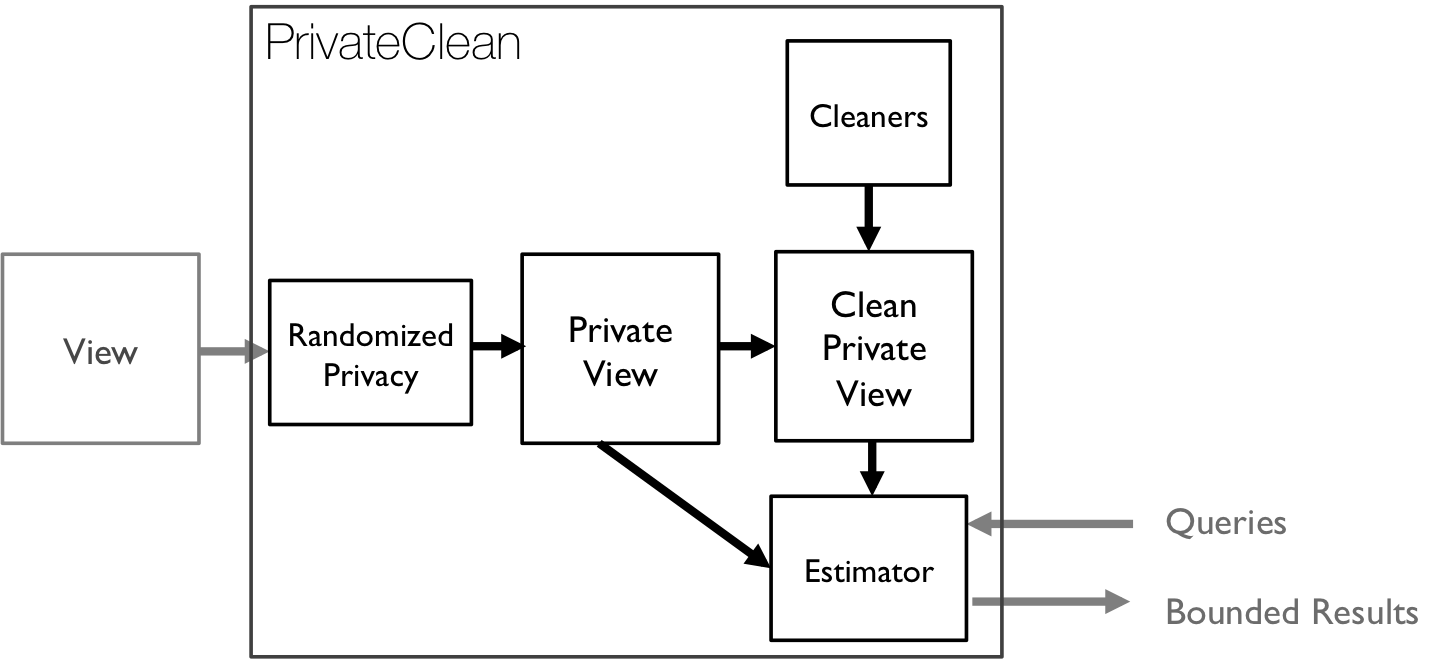
\includegraphics[width=\columnwidth]{figs/architecture.png}
 \caption{The architecture of \sys \label{architecture}}
\end{figure}
